\documentclass{report}
\usepackage[a4paper, margin=1.5in]{geometry}
\usepackage[utf8]{inputenc}
\usepackage{array}
\usepackage{tikz}
\usepackage{color}
\usepackage{hyperref}
\usepackage{graphicx}
\usepackage{float}
% \usepackage{algorithm}
%\usepackage{algorithmic}
\usepackage{listings}
\usepackage{amsmath}
\usepackage[noend]{algpseudocode}
\usepackage[linesnumbered,noline,noend]{algorithm2e}
\usepackage{subfiles}

\newcommand{\RNum}[1]{\uppercase\expandafter{\romannumeral #1\relax}}
\newcolumntype{L}[1]{>{\raggedright\let\newline\\\arraybackslash\hspace{0pt}}m{#1}}
\newcolumntype{C}[1]{>{\centering\let\newline\\\arraybackslash\hspace{0pt}}m{#1}}
\newcolumntype{R}[1]{>{\raggedleft\let\newline\\\arraybackslash\hspace{0pt}}m{#1}}


\SetNlSty{}{}{}

\let\oldnl\nl% Store \nl in \oldnl
\newcommand\nonl{%
	\renewcommand{\nl}{\let\nl\oldnl}}% Remove line number for one line


\title{
	\line(1,0){300}
	\endgraf\bigskip
	\Huge
	\emph{Digital Modulation\\Amplitude Shift Keying\\
		\hspace{1.1cm}Frequency Shift Keying}
	\newline
	\line(1,0){300}
	\bigskip
	\bigskip
}

\author{
	\Large{Sihat Afnan}\\
	\Large{Student ID : 1705098}\\\\
	\Large{Farhana Khan}\\
	\Large{Student ID : 1705100}
}

\date{
	\endgraf\bigskip
	\Large{\today}
}

\newcommand{\TripleRowDoubleCol}[6]{
	\begin{center}
		\begin{tabular}{|c|c|}
			\hline
			#1 & #2\\\hline
			#3 & #4\\\hline
			#5 & #6\\\hline
		\end{tabular}
	\end{center}
}

\begin{document}
	
	\maketitle
	\renewcommand{\familydefault}{\sfdefault}
	
	\tableofcontents
	
	\chapter{Introduction}
	Digital communication is imperative in data communication.It is extensively used as it provides many advantages over analog communication.Digital communication methods are more immune to noise-related problems than analog communications.This communication system is comparatively low in cost than the analog communication system.Due to the presence of digitized signal, coding can be implemented which is not achievable in analog communication due to analog nature of the signal being transmitted.Distortion-less regenerative repeaters can be employed between transmitter and receiver in digital communication methods which is also not possible in analog communication.\bigskip
	
	However, the main challenge of digital communication is that, digital signals cannot be directly transmitted.It requires an analog carrier wave for its transmission. The process of encoding a digital information signal into an analog carrier wave, by modifying its different properties such as, the amplitude, phase, or frequency is called Digital Modulation.This analog carrier wave is the transmitted signal of the data communication required. In addition to transmission of digital data, complex modulation schemes allow us to pack more bits in each transmitted symbol hence achieving higher data transfer speeds.Thus, this encoding process also affects the bandwidth of the transmitted signal and required channel properties.\bigskip
	
	Many techniques of digital modulation, from traditional techniques such as ASK, FSK, BPSK, QPSK and QAM to the most recent techniques such as MSK, CPM and MHPM and more, are prevalent in today's digital communication.Among these, ASK and FSK are the topics of interest.
	
	\newpage
	
	\chapter{Amplitude Shift keying}
	
	\section{Introduction}
	\bigskip
	Amplitude-shift keying (ASK) is the simplest digital modulation technique.In ASK, digital data is represented as variations in the amplitude of a carrier wave.A carrier wave with constant amplitude and fixed frequency is used.Whose amplitude is then decreased or increased according to the digital data, which is required to be transmitted.  
	
	Any digital modulation scheme uses a finite number of distinct signals to represent digital data. ASK uses a finite number of amplitudes, each represents an unique level or state of the digital data. 
	
	\section{ASK Modulation}
	
	In ASK modulation, a carrier signal generator and a band-pass filter is required. The carrier generator, sends a continuous high-frequency carrier, which then modified by the binary sequence (message signal). 
	The band-pass filter, which is basically a  pulse-shaping filter, shapes the pulse depending according to its amplitude and phase characteristics.\bigskip
	
	
	\begin{figure}[H]
		\centering
		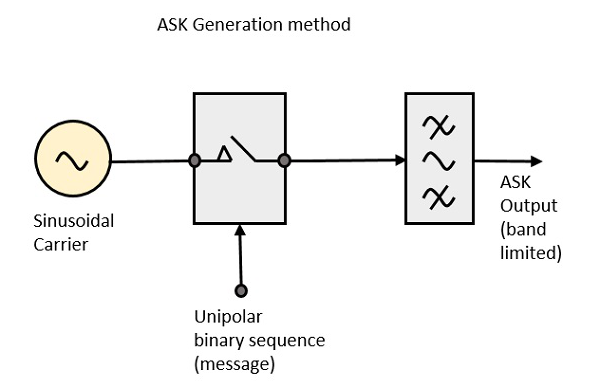
\includegraphics[scale=0.5]{images/ask_modulator.jpg}
		\caption{ASK Modulator}
	\end{figure}	
	
	\bigskip

	\begin{figure}[h]
		\centering
		
		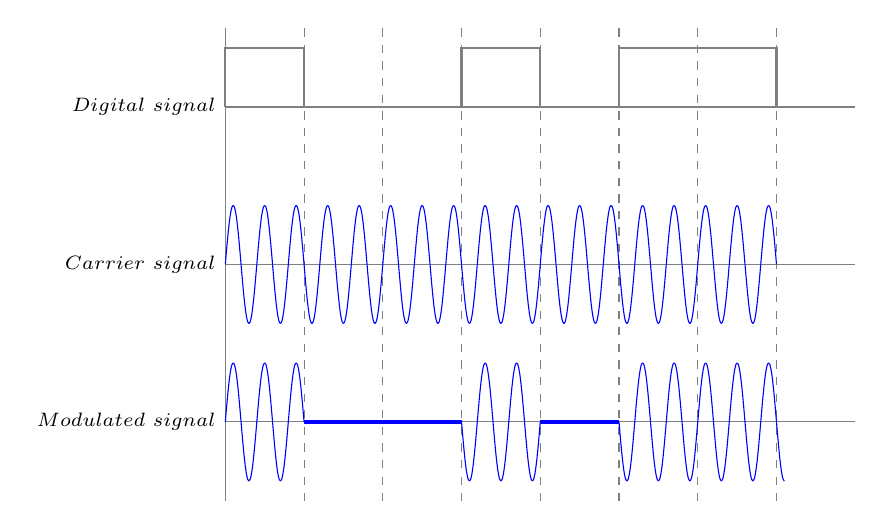
\begin{tikzpicture}
			\draw[gray] (0, 3) -- (0, -3);		% y axis
			\draw (0, 2) node[left,font=\scriptsize] {$Digital\hspace{0.1cm}signal$};
			\draw[gray]	(0, 2) -- (8, 2);		% x axis for digital signal
			\draw (0, 0) node[left,font=\scriptsize] {$Carrier\hspace{0.1cm}signal$};
			\draw[gray]	(0, 0) -- (8, 0);		% x axis for carrier signal
			\draw (0, -2) node[left,font=\scriptsize] {$Modulated\hspace{0.1cm}signal$};
			\draw[gray]	(0, -2) -- (8, -2);		% x axis for modulated signal
			
			\draw[gray, dashed, xshift=1cm] (0, 3) -- (0, -3);
			\draw[gray, dashed, xshift=2cm] (0, 3) -- (0, -3);
			\draw[gray, dashed, xshift=3cm] (0, 3) -- (0, -3);
			\draw[gray, dashed, xshift=4cm] (0, 3) -- (0, -3);
			\draw[gray, dashed, xshift=5cm] (0, 3) -- (0, -3);
			\draw[gray, dashed, xshift=6cm] (0, 3) -- (0, -3);
			\draw[gray, dashed, xshift=7cm] (0, 3) -- (0, -3);
			
			% drawing digital signal
			\draw[gray, thick] (0,2) -- (0,2.75) -- (0,2.75) -- (1,2.75) -- (1,2.75) -- (1,2);
			
			\draw[gray, thick] (1,2) -- (3,2);
			
			\draw[gray, thick] (3,2) -- (3,2.75) -- (3,2.75) -- (4,2.75) -- (4,2.75) -- (4,2);
			
			\draw[gray, thick] (4,2) -- (5,2);
			
			\draw[gray, thick] (5,2) -- (5,2.75) -- (5,2.75) -- (7,2.75) -- (7,2.75) -- (7,2);
			
			% drawing  carrier signal
			\foreach \x in {0,0.4,...,7}{
				\draw[blue] (\x,0) sin (0.1 + \x, 0.75) ;
			}
			
			\foreach \x in {0.1,0.5,...,7}{
				\draw[blue] (\x,0.75) cos (0.1 + \x, 0) ;
			}
			
			\foreach \x in {0.2,0.6,...,7}{
				\draw[blue] (\x,0) sin (0.1 + \x, -0.75) ;
			}
			
			\foreach \x in {0.3,0.7,...,7}{
				\draw[blue] (\x,-0.75) cos (0.1 + \x, 0) ;
			}
			
			% drawing  modulated signal
			\foreach \x in {0,0.4,...,1}{
				\draw[blue] (\x,-2) sin (0.1 + \x, -1.25) ;
			}
			
			\foreach \x in {0.1,0.5,...,1}{
				\draw[blue] (\x,-1.25) cos (0.1 + \x, -2);
			}
			
			\foreach \x in {0.2,0.6,...,1}{
				\draw[blue] (\x,-2) sin (0.1 + \x, -2.75) ;
			}
			
			\foreach \x in {0.3,0.7,...,1}{
				\draw[blue] (\x,-2.75) cos (0.1 + \x, -2);
			}	
			%__________
			\draw[blue, ultra thick, yshift=-4cm]  (1,2) -- (3,2);
			
			\foreach \x in {3.2,3.6,...,4}{
				\draw[blue] (\x,-2) sin (0.1 + \x, -1.25) ;
			}
			
			\foreach \x in {3.3,3.7,...,4}{
				\draw[blue] (\x,-1.25) cos (0.1 + \x, -2);
			}
			
			\foreach \x in {3,3.4,...,4}{
				\draw[blue] (\x,-2) sin (0.1 + \x, -2.75) ;
			}
			
			\foreach \x in {3.1,3.5,...,4}{
				\draw[blue] (\x,-2.75) cos (0.1 + \x, -2);
			}		
			%__________
			\draw[blue, ultra thick, yshift=-4cm] (4,2) -- (5,2);
			
			\foreach \x in {5.2,5.6,...,7}{
				\draw[blue] (\x,-2) sin (0.1 + \x, -1.25) ;
			}
			
			\foreach \x in {5.3,5.7,...,7}{
				\draw[blue] (\x,-1.25) cos (0.1 + \x, -2);
			}
			
			\foreach \x in {5,5.4,...,7}{
				\draw[blue] (\x,-2) sin (0.1 + \x, -2.75) ;
			}
			
			\foreach \x in {5.1,5.5,...,7}{
				\draw[blue] (\x,-2.75) cos (0.1 + \x, -2);
			}	
			
		\end{tikzpicture}
		
		\caption{Binary signal modulation with ASK}
	\end{figure}

	\bigskip
	
	Figure 2.2 demonstrates an example of applying Amplitude Shift Keying on a binary level digital signal. It is observable from the figure that the modulated signal remains on and off for different intervals on the time axis, according to the message signal. Hence, this is also known as On/Off keying (OOK). This same encoding method can be applied to multi-level message signals as well. The number of unique amplitudes of the final modulated signal will be equal to the number of different levels the message signal has.
	\\
	\bigskip
	
		\begin{figure}[h]
		\centering
		
		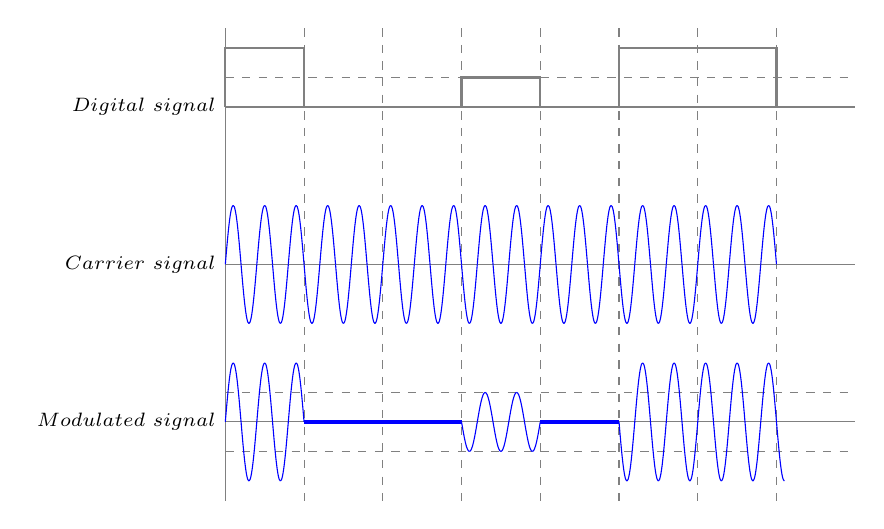
\begin{tikzpicture}
			\draw[gray] (0, 3) -- (0, -3);		% y axis
			\draw (0, 2) node[left,font=\scriptsize] {$Digital\hspace{0.1cm}signal$};
			\draw[gray]	(0, 2) -- (8, 2);		% x axis for digital signal
			\draw (0, 0) node[left,font=\scriptsize] {$Carrier\hspace{0.1cm}signal$};
			\draw[gray]	(0, 0) -- (8, 0);		% x axis for carrier signal
			\draw (0, -2) node[left,font=\scriptsize] {$Modulated\hspace{0.1cm}signal$};
			\draw[gray]	(0, -2) -- (8, -2);		% x axis for modulated signal
			
			\draw[gray, dashed, xshift=1cm] (0, 3) -- (0, -3);
			\draw[gray, dashed, xshift=2cm] (0, 3) -- (0, -3);
			\draw[gray, dashed, xshift=3cm] (0, 3) -- (0, -3);
			\draw[gray, dashed, xshift=4cm] (0, 3) -- (0, -3);
			\draw[gray, dashed, xshift=5cm] (0, 3) -- (0, -3);
			\draw[gray, dashed, xshift=6cm] (0, 3) -- (0, -3);
			\draw[gray, dashed, xshift=7cm] (0, 3) -- (0, -3);
			
			\draw[gray, dashed, yshift=2.375cm] (0, 0) -- (8, 0);
			\draw[gray, dashed, yshift=-2.375cm] (0, 0) -- (8, 0);
			\draw[gray, dashed, yshift=-1.625cm] (0, 0) -- (8, 0);
			
			% drawing digital signal
			\draw[gray, thick] (0,2) -- (0,2.75) -- (0,2.75) -- (1,2.75) -- (1,2.75) -- (1,2);
			
			\draw[gray, thick] (1,2) -- (3,2);
			
			\draw[gray, thick] (3,2) -- (3,2.375) -- (3,2.375) -- (4,2.375) -- (4,2.375) -- (4,2);
			
			\draw[gray, thick] (4,2) -- (5,2);
			
			\draw[gray, thick] (5,2) -- (5,2.75) -- (5,2.75) -- (7,2.75) -- (7,2.75) -- (7,2);
			
			% drawing  carrier signal
			\foreach \x in {0,0.4,...,7}{
				\draw[blue] (\x,0) sin (0.1 + \x, 0.75) ;
			}
			
			\foreach \x in {0.1,0.5,...,7}{
				\draw[blue] (\x,0.75) cos (0.1 + \x, 0) ;
			}
			
			\foreach \x in {0.2,0.6,...,7}{
				\draw[blue] (\x,0) sin (0.1 + \x, -0.75) ;
			}
			
			\foreach \x in {0.3,0.7,...,7}{
				\draw[blue] (\x,-0.75) cos (0.1 + \x, 0) ;
			}
			
			% drawing  modulated signal
			\foreach \x in {0,0.4,...,1}{
				\draw[blue] (\x,-2) sin (0.1 + \x, -1.25) ;
			}
			
			\foreach \x in {0.1,0.5,...,1}{
				\draw[blue] (\x,-1.25) cos (0.1 + \x, -2);
			}
			
			\foreach \x in {0.2,0.6,...,1}{
				\draw[blue] (\x,-2) sin (0.1 + \x, -2.75) ;
			}
			
			\foreach \x in {0.3,0.7,...,1}{
				\draw[blue] (\x,-2.75) cos (0.1 + \x, -2);
			}	
			%__________
			\draw[blue, ultra thick, yshift=-4cm]  (1,2) -- (3,2);
			
			\foreach \x in {3.2,3.6,...,4}{
				\draw[blue] (\x,-2) sin (0.1 + \x, -1.625) ;
			}
			
			\foreach \x in {3.3,3.7,...,4}{
				\draw[blue] (\x,-1.625) cos (0.1 + \x, -2);
			}
			
			\foreach \x in {3,3.4,...,4}{
				\draw[blue] (\x,-2) sin (0.1 + \x, -2.375) ;
			}
			
			\foreach \x in {3.1,3.5,...,4}{
				\draw[blue] (\x,-2.375) cos (0.1 + \x, -2);
			}		
			%__________
			\draw[blue, ultra thick, yshift=-4cm] (4,2) -- (5,2);
			
			\foreach \x in {5.2,5.6,...,7}{
				\draw[blue] (\x,-2) sin (0.1 + \x, -1.25) ;
			}
			
			\foreach \x in {5.3,5.7,...,7}{
				\draw[blue] (\x,-1.25) cos (0.1 + \x, -2);
			}
			
			\foreach \x in {5,5.4,...,7}{
				\draw[blue] (\x,-2) sin (0.1 + \x, -2.75) ;
			}
			
			\foreach \x in {5.1,5.5,...,7}{
				\draw[blue] (\x,-2.75) cos (0.1 + \x, -2);
			}	
			
		\end{tikzpicture}
		
		\caption{Multilevel signal modulation with ASK}
	\end{figure}

	\bigskip
	\newpage
	
	
	\section{ASK Demodulation}
	\bigskip 
	
	The Demodulator of ASK is designed specifically for the symbol-set used by the modulator. It determines the amplitude of the received signal and maps it back to the symbol it represents. Thus, the original message signal is recovered. Frequency and phase of the carrier are considered constant.
	
	There are two ways of ASK demodulation. They are,
	\begin{enumerate}
		\item Coherent Detection
		\item Non coherent Detection
	\end{enumerate}
	\bigskip
	
	\subsection{Coherent Detection}
	
	\bigskip
	
	
	\begin{figure}[H]
		\centering
		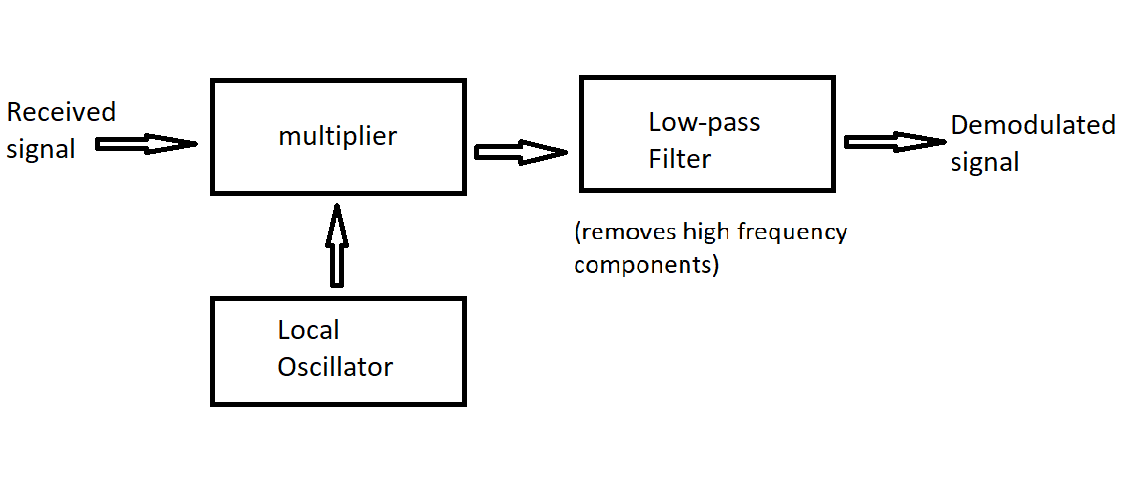
\includegraphics[scale=0.4]{images/synchronous_detector.png}
		\caption{ASK Demodulator: Coherent}
	\end{figure}	
	
	\bigskip
	
	The ASK modulated waveform received from the channel by the receiver is passed through a multiplier circuit. The output of the multiplier is forwarded to the low pass filter to eliminate noise and unnecessary low and high frequency components. 
	\bigskip
	
	This is a synchronous method and therefore very effective. A local oscillator is used for this synchronization purpose. But this also increases the total cost of demodulation.
	
	\bigskip
	\newpage
	\subsection{Non Coherent Detection}
	
	\bigskip
	
	
	\begin{figure}[H]
		\centering
		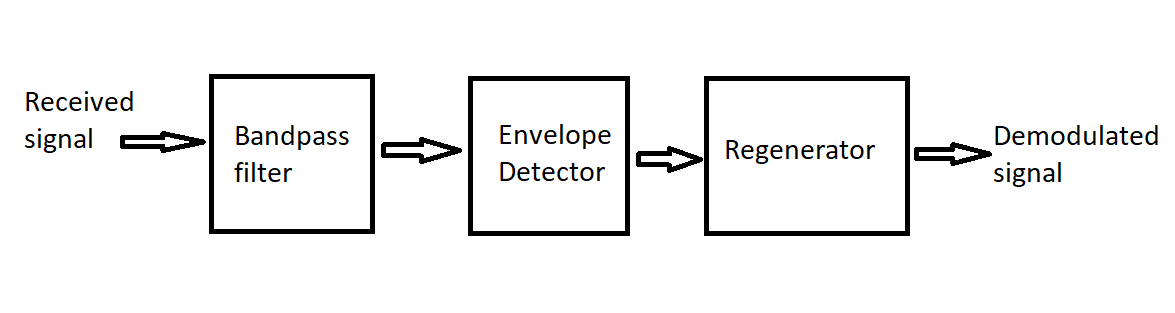
\includegraphics[scale=0.4]{images/asynchronous_detector.png}
		\caption{ASK Demodulator: Non Coherent}
	\end{figure}	
	
	\bigskip
	
	In this method the ASK modulated waveform is passed through a band-pass filter and then to the Envelope Detector. The output of the Envelope Detector is forwarded to a regenerator to generate the demodulated message signal. 
	\bigskip
	
	This method is cost effective as no oscillator is being used. It is an asynchronous method. In spite of its success in cost reduction, this method is more noise prone compared to the coherent method and hence we get a low SNR (Signal to Noise Ratio).
	
	\bigskip
	
	
	\section{Applications of ASK}
	\bigskip
	
	There are many applications of Amplitude Shift Keying. Such as,
	\begin{itemize}
		\item In ASK modulation a very high frequency carrier wave is used, which provides a wide broadcasting range. Therefore, ASK modulated digital signals can be broadcasted.
		\item In optical fiber communication for LASER intensity modulation ASK is very commonly used.
		\item ASK modulation can also be used for transmitting Morse Codes.
		
	\end{itemize}
	
	\newpage
	
	\chapter{Frequency Shift Keying}
	\section{Introduction}{
		\bigskip
		
	Frequency Shift Keying (FSK) is the digital modulation technique in which the frequency of the carrier signal varies according to the digital signal changes. FSK is a scheme of frequency modulation.\bigskip
	
	The output of a FSK modulated wave is high in frequency for a binary High input and is low in frequency for a binary Low input. The binary 1s and 0s are called Mark and Space frequencies.\bigskip
	
	The following image is the diagrammatic representation of FSK modulated waveform along with its input.
		\bigskip
		
\begin{figure}[H]
	\centering
	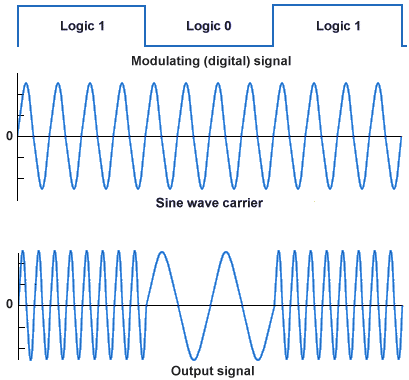
\includegraphics[scale=0.8]{images/2.png}
	\caption{Diagrammatic Representation of FSK}
	\label{fig:}
\end{figure}
	}
	
	\section{FSK Modulator}{
		\bigskip
		In FSK, the binary information can be transmitted through a carrier signal along with frequency changes. The below diagram shows the frequency shift keying block diagram.\bigskip
		
		\begin{figure}[H]
			\centering
			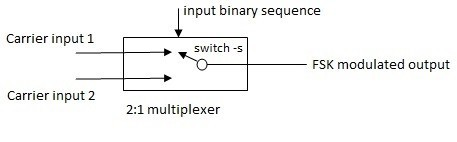
\includegraphics{images/fsk_bd.jpg}
			\caption{Block Diagram of FSK modulator}
			\label{fig:}
		\end{figure}
		
		In FSK, two carrier signals are used to produce FSK modulated waveforms. The reason behind this, FSK modulated signals are represented in terms of two different frequencies. The frequencies are called “mark frequency” and “space-frequency”. Mark frequency has represented logic 1 and space-frequency has represented the logic 0. There is only one difference between these two carrier signals, i.e. carrier input 1 having more frequency than the carrier input 2.\bigskip 
		
		The switch (s) of the 2:1 multiplexer is having the important role to generate the FSK output. Here the switch is connected to carrier input 1 for all logic 1’s of the binary input sequence. And switch (s) is connected to carrier input 2 for all logic 0’s of the input binary sequence. So, the resultant FSK modulated waveforms have mark frequencies and space frequencies.\bigskip 
		
			
		\begin{figure}[H]
			\centering
			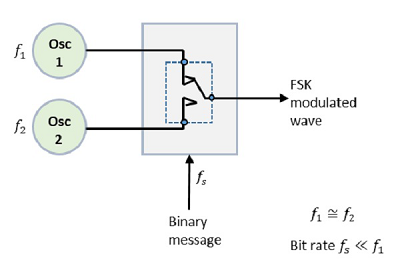
\includegraphics{images/fsk_transmitter.jpg}
			\caption{FSK Transmitter}
			\label{fig:}
		\end{figure}	
		
		
		\bigskip
	}
\newpage

\section{Classification of FSK}{
	\bigskip
	Based on the number of discrete frequencies , There can be two types of FSK schemes.
	\begin{enumerate}
		\bigskip
		\item {\textbf{BFSK :} This scheme has only two discrete frequencies,which was discussed previously.One is known as Mark,another is known as Space.}
		\item {\textbf{MFSK :} This scheme has more than two discrete frequencies.}
		
	\end{enumerate}    
	Apart from this classification,there can be another FSK schemes,\textbf{Minimum shift Keying} (MSK) , which is a type of continuous-phase frequency-shift keying.
		
}

	\section{BFSK}{
	\bigskip
	BFSK is the most widely used FSK schemes.In this scheme,the number of discrete frequencies is two.The two binary states, logic 0 (low) and 1 (high), are each represented by an Analog waveform. Logic 0 is represented by a wave at a specific frequency, and logic 1 is represented by a wave at a different frequency.\bigskip
	
	\begin{figure}[H]
		\centering
		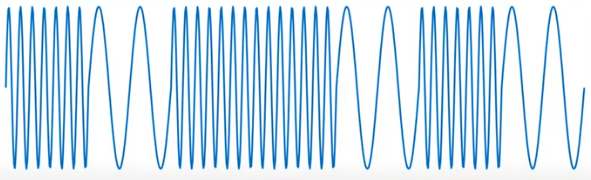
\includegraphics[width=\linewidth]{images/1.png}
		\caption{Two discrete frequencies of BFSK}
		\label{fig:}
	\end{figure}
	
	Binary FSK is a constant-envelope form of angle modulation similar to conventional frequency modulation except that the modulating signal varies between two discrete voltage levels (i.e., 1’s and 0’s) rather than with a continuously changing value, such as a sine wave.\bigskip
	
	With binary FSK, the center or carrier frequency is shifted by the binary input signal. Consequently, the output from an FSK modulator is a step function in the frequency domain. As the binary input signal changes from a logic 0 to logic 1 and vice versa, the FSK output signal shifts between two frequencies.
	
	\newpage
	
	\subsection{Tone Spacing}
	 \bigskip 
	  An  important  question  in  FSK is how far apart the mark and space should be placed.To be more precise, what value of deviation should we use?If the two  tones  are  too  close  together  they  could  interfere with each  other and create \textbf{intersymbol interference}.
	  
	  \begin{figure}[H]
	  	\centering
	  	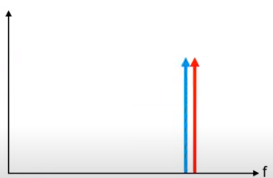
\includegraphics{images/8.png}
	  	\caption{Intersymbol Interference}
	  	\label{fig:}
	  \end{figure}
  
	  If they are too far apart, this is spectrally inefficient because in that case the signal uses \textbf{too much bandwidth}.
	  
	  \begin{figure}[H]
	  	\centering
	  	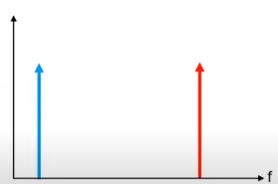
\includegraphics{images/9.png}
	  	\caption{Excessive Bandwith Consumption}
	  	\label{fig:}
	  \end{figure}
	  
	  
	  To minimize the bandwidth of the FSK signal the tone should be asclose to each other as possible without creating inter symbol interference
	 \subsection{Bandwith}
	 \bigskip
	 BFSK bandwith depends on both
	 \begin{itemize}
	 	\item Frequency deviation
	 	\item Bit rate of data
	 \end{itemize}
 	  
 	 \newpage 
 	  
	 Although it might seem that the total bandwidth of an FSK signal is simply twice the frequency deviation this would be incorrect.The minimum FSK bandwidth is actually a function of both the frequency deviation and the bit rate of the modulating signal.The formula for minimum FSK bandwidth is two times the sum of the deviation and the bit rate.
	 \begin{center}
	 	BFSK Bandwith = $2(F_d + F_b)$
	 \end{center}
	 
	 \subsection{Modulation Index}
	 \bigskip
	 Modulation index (H) is the ratio of twice the deviation to the bit rate.In essence,it is a measurement of how far apart, the two tones should be.
	 
	 \begin{center}
	 	 $H = \frac{2*F_d}{F_b}$  
	 \end{center}
	 
	 For example if we are using a deviation of 20 kilohertz and the bit rate is 40 kilobits per second, then we have a modulation index of 1.0.If we were to decrease the deviation to only 10 kilohertz, that is move the tones closer together, the modulation index would decrease to 0.5.Optimal detection of a received FSK signal occurs when the  modulation  index  H  is  greater  than  1.Some coherent FSK schemes like MSK(Minimum  Shift Keying) can detect signal with H=0.5.Therefore,we can say that MSK needs less bandwith than BFSK to reliably transmit signal at the same bit rate.
	 
}
	
	\section{M-ary FSK}
	\bigskip 
	Multiple frequency-shift keying (MFSK) is a variation of frequency-shift keying (FSK) that uses more than two frequencies. MFSK is a form of M-ary orthogonal modulation, where each symbol consists of one element from an alphabet of orthogonal waveforms. M, the size of the alphabet, is usually a power of two so that each symbol represents $\log_2(M)$ bits.
	
	\begin{figure}[H]
		\centering
		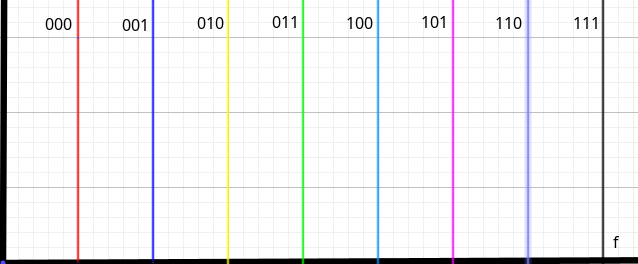
\includegraphics[width=\linewidth]{images/mfsk.png}
		\caption{MFSK frequencies}
		\label{fig:}
	\end{figure}

\newpage

	\section{Minimum Shift Keying}
	Minimum shift keying, MSK, is a form frequency modulation based on a system called continuous-phase frequency-shift keying.
	Minimum shift keying, MSK offers advantages in terms of spectral efficiency when compared to other similar modes, and it also enables power amplifiers to operate in saturaton enabling them to provide high levels of efficiency.\bigskip
	
	It is found that binary data consisting of sharp transitions between "one" and "zero" states and vice versa potentially creates signals that have sidebands extending out a long way from the carrier, and this creates problems for many radio communications systems, as any sidebands outside the allowed bandwidth cause interference to adjacent channels and any radio communications links that may be using them.	
	MSK, minimum shift keying has the feature that there are no phase discontinuities and this significantly reduces the bandwidth needed over other forms of phase and frequency shift keying.\bigskip 
	
	The problem can be overcome in part by filtering the signal, but is found that the transitions in the data become progressively less sharp as the level of filtering is increased and the bandwidth reduced. To overcome this problem GMSK is often used and this is based on Minimum Shift Keying, MSK modulation. The advantage of which is what is known as a continuous phase scheme. Here there are no phase discontinuities because the frequency changes occur at the carrier zero crossing points.\\
	
	\begin{figure}[H]
		\centering
		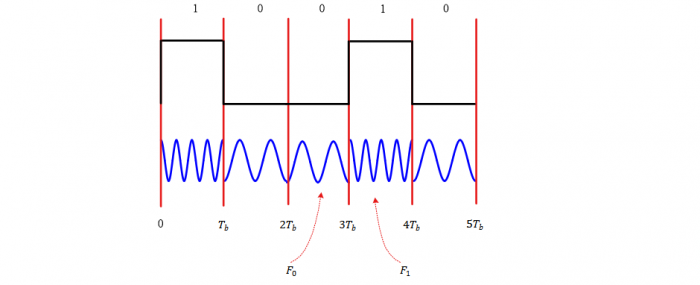
\includegraphics[width=\linewidth]{images/msk.png}
		\caption{Minimum Shift Keying}
		\label{fig:}
	\end{figure}
	
	When looking at a plot of a signal using MSK modulation, it can be seen that the modulating data signal changes the frequency of the signal and there are no phase discontinuities. This arises as a result of the unique factor of MSK that the frequency difference between the logical one and logical zero states is always equal to half the data rate. This can be expressed in terms of the modulation index, and it is always equal to 0.5.
	
	\newpage
	
	\section{Demodulation of FSK}
	\bigskip 
	Demodulation is defined as reconstructing the original signal from the modulated signal. This demodulation can be possible in two ways. They are
	
	\begin{itemize}
		\item Coherent FSK detection
		\item Non-coherent FSK detection
	\end{itemize}

	The only difference between the coherent and non-coherent way of detection is the phase of the carrier signal. If the carrier signal we are using at the transmitter side and receiver side are in the same phase while demodulation process i.e. called a coherent way of detection and it is also known as synchronous detection. If the carrier signals which we are using at transmitter and receiver side are not in the same phase then such modulation process known as Non-coherent detection. Another name for this detection is Asynchronous detection.
	
	\subsection{Coherent FSK detection}
	In this synchronous FSK detection, the modulated wave got affected by noise while reaching the receiver. So, this noise can be eliminated from using the bandpass filter (BPF). Here at multiplier stage, the noisy FSK modulated signal is multiplied with the carrier signal from the local oscillator device. Then the resultant signal passes from the BPF. Here this bandpass filter is assigned to cut off frequency which is equal to the binary input signal frequency. So the same frequencies can be allowed to the decision device. Here this decision device gives 0 and 1 for space and mark frequencies of the FSK modulated waveforms.
	
	\begin{figure}[H]
		\centering
		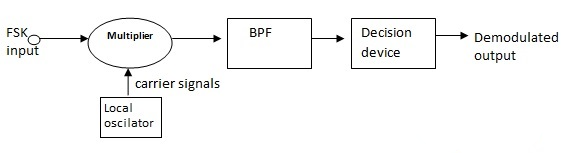
\includegraphics[width=\linewidth]{images/coherent_fsk.png}
		\caption{Coherent FSK Detection}
		\label{fig:}
	\end{figure}

	\subsection{Non-coherent FSK Detection}
	\bigskip
	The modulated FSK signal is forwarded from the bandpass filter 1 and 2 with cut off frequencies equals to space and mark frequencies. So, the unwanted signal components can be eliminated from the BPF. And the modified FSK signals are applied as input to the two envelop detectors. This envelope detector is a circuit having a diode (D).
	
	\newpage
	
		\begin{figure}[H]
		\centering
		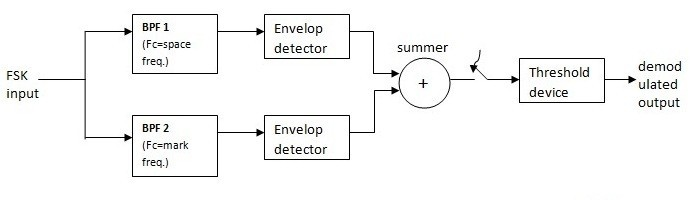
\includegraphics[width=\linewidth]{images/non_coherent_fsk.jpg}
		\caption{Non-Coherent FSK Detection}
		\label{fig:}
	\end{figure}
	
	Based upon the input to the envelope detector it delivers the output signal. This envelope detector used in the amplitude demodulation process. Based upon its input it generates the signal and then it is forwarded to the threshold device. This threshold device gives the logic 1 and 0 for the different frequencies. This would be equal to the original binary input sequence. So, the FSK generation and detection can be done in this way. This process can be known for the frequency-shift keying modulation and demodulation experiment also. In this FSK experiment, FSK can be generated by the 555 timer IC and detection can be possible by 565IC which is known as a phase-locked loop (PLL).


	\section{Applications of FSK}
	\bigskip
	Following are some typical application of Frequency Shift Keying
	\begin{itemize}
		\item It is used on voice grade lines for data rates upto 1200 bps.
		\item It is used for high frequency radio transmission from 3 to 30 MHz.
		\item It is also used in coaxial cable based LAN (Local Area Network) at higher frequencies.
		\item FSK schemes are used in amplifier design and simplification.
		\item Paging systems in digital communication technology is an acknowledged field where FSK schemes are being used.
		\item FSK is also used in data collection(metering) and radio communication systems.
	\end{itemize}

	
\chapter{Conclusion}
\bigskip 
We have tried to give a general overview of two digital modulation techniques,Amplitude Shift Keying and Frequency Shift Keying in this report.However,as you might have already noticed,the volume of contents on Frequency Shift Keying is comparatively larger since we have discussed some of its classifications unlike Amplitude Shift Keying.After giving a general introduction of the said two methods,we have dived deep into the modulation and demodulation techniques.\bigskip 

However,our report doesn't deal with the mathematical analyses behind such modulation techniques.Since our main purpose was to come up with an overview of ASK and FSK,we avoided the mathematics behind probability of error,noise effect,inter symbol interference etc. which, we presumed, would make the report more tedious to go through.Apart from that,we included several figures to make the readers understand modulation and demodulation process clearly.   



\end{document}